\section{Desenvolvimento}

% =====#=====#=====#===== %

\subsection{Hardware e Plataforma de Validação}
O sistema emprega um módulo GY-521 com sensor MPU-6050 (ADC de 16 bits por eixo) \cite{5.invensense2013spec} conectado a um ESP32 DevKit (Arduino IDE) via IC a 400 KHZ (endereço 0x68, GPIO 21/SDA e GPIO 22/SCL). Embora a escala de $\pm 2 \text{ g}$ (16384 LSB/g) maximize a resolução nominal, testes preliminares identificaram offset superior a +1,3 g no eixo \textbf{X}, o que causaria saturação em +1 g ($+2,3 \text{ g} > 2 \text{ g}$). Configurou-se, portanto, o registrador ACCEL\_Config (0x1C) para $\pm 4 \text{ g}$ (AFS\_SEL = 1; 8192 LSB/g, resolução melhor qye 0,01°/LSB), com filtro DLPF em 5 Hz (CONFIG = 0x06) e amostragem de 100 Hz (SMPLRT\_DIV = 0x09) \cite{6.invensense2013register}. 

A Figura~\ref{fig:estrutura} Apresenta a estrutura articulada impressa em 3D com dois níveis bolha ortogonais embutidos no bloco do GY-521 para auxiliar o nivelamento \cite{4.ochoa2026} e o transferido de 0° a 180° acoplado lateralmente para validação em um grau de liberdade.

\begin{figure}[h]
    \centering

    \begin{subfigure}{0.3\textwidth}
        \centering
        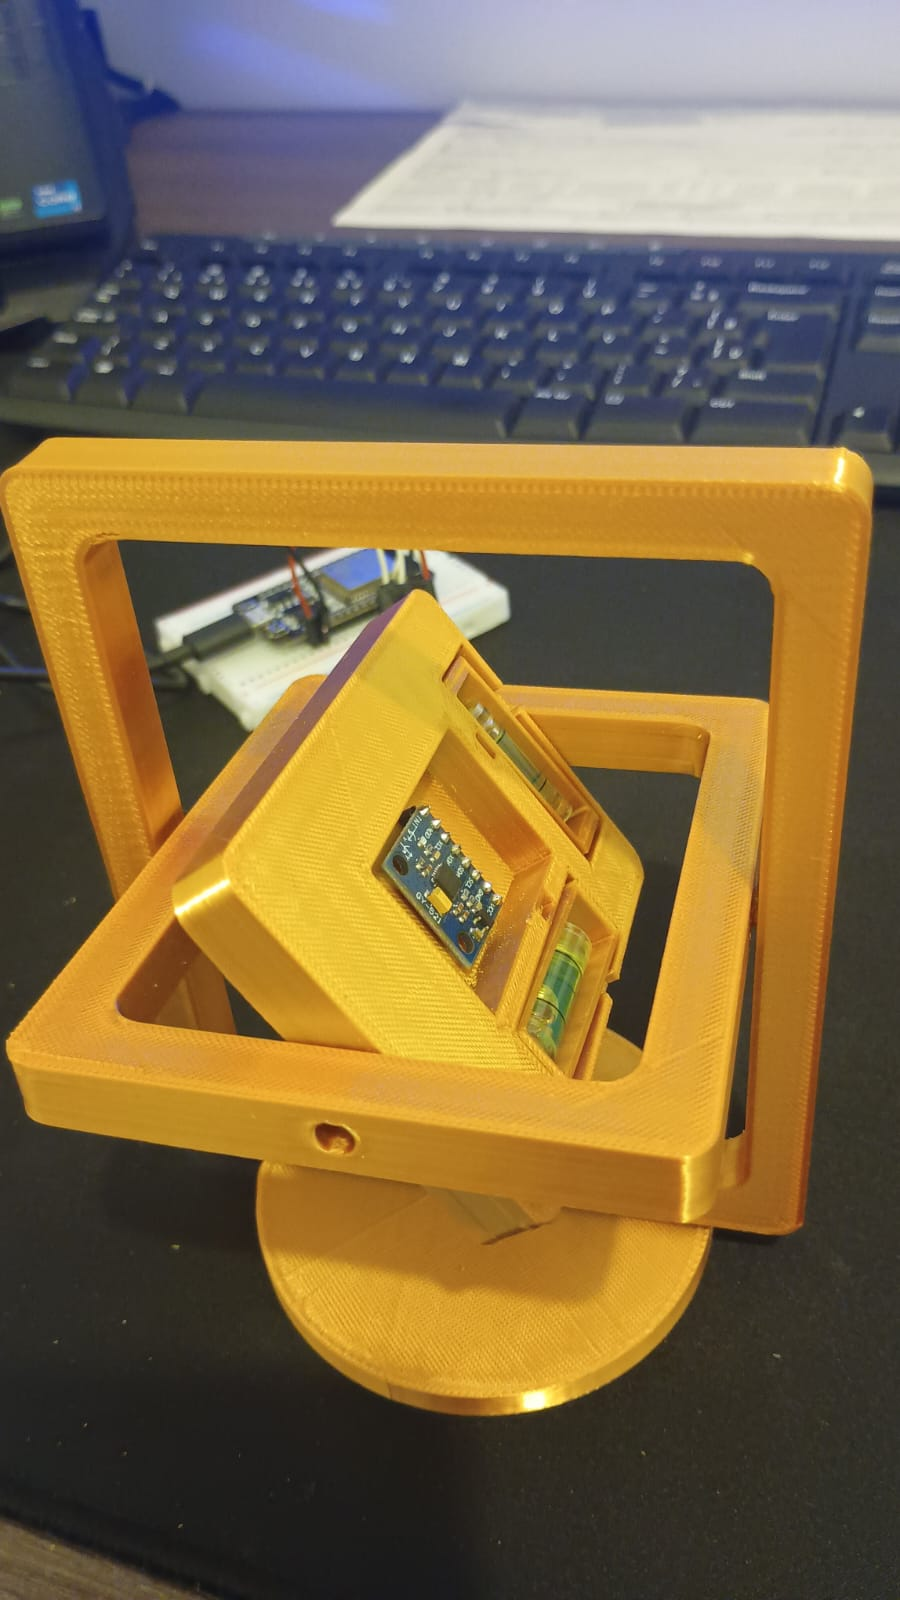
\includegraphics[width=\textwidth]{IMG/plataforma.jpeg}
        \caption{Suporte 3D com GY-521}
        \label{fig:imagem1}
    \end{subfigure}
    \hspace{0.5cm}
    \begin{subfigure}{0.3\textwidth}
        \centering
        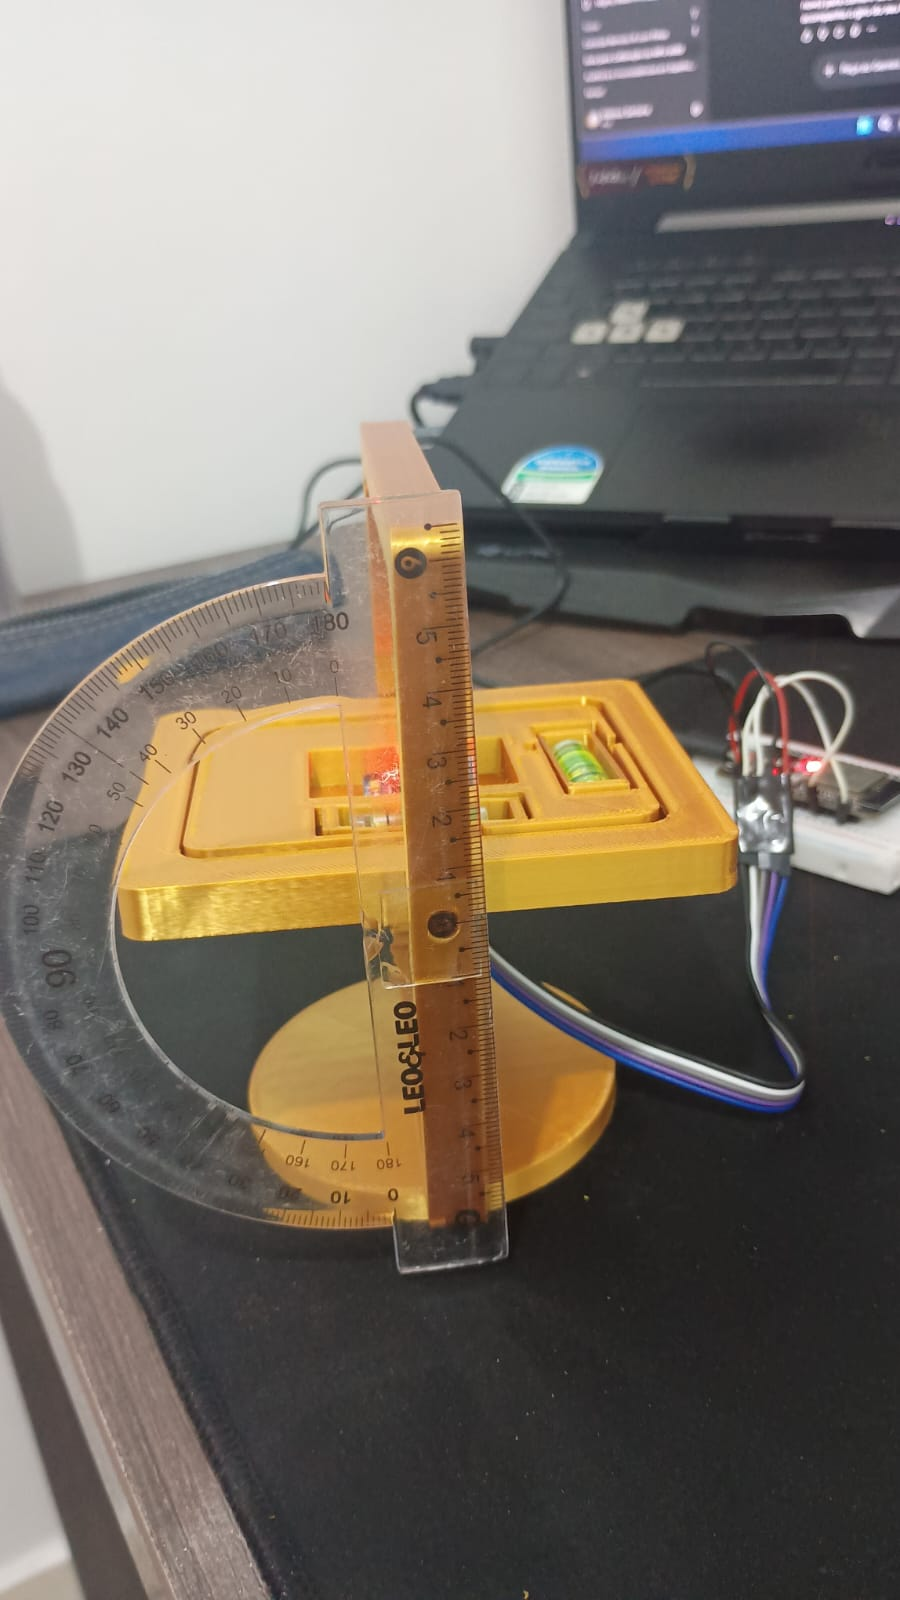
\includegraphics[width=\textwidth]{IMG/sistema.jpeg}
        \caption{Transferidor em 90°}
        \label{fig:imagem2}
    \end{subfigure}

    \vspace{0.2cm}

    \caption{Aparato experimental: (a) plataforma 3D com GY-521, níveis bolha e ESP32 ao fundo; (b) conjunto com transferidor (0° a 180°) na referência horizontal de 90°.}
    \label{fig:estrutura}
\end{figure}

% =====#=====#=====#===== %

\subsection{Calibração Estática do Acelerômetro}
Modelou-se a saída estática de cada eixo $i \in \{X, Y, Z\}$ em [$g$] por uma relação linear frente à aceleração de referencia $A_{ref}$ \cite{4.ochoa2026}

\begin{equation}
    A_{saída} = Ganho_i \times A_{ref} \times A_{offset,i}
    \label{eq:equacao_1}
\end{equation}

Alinhando cada eixo às seis orientações ortogonais ($\pm 1 \text{ g}$) sobre superfície nivelada e coletando N=200 amostras por posição (acima do mínimo de 100 exigidos \cite{4.ochoa2026}), obtiveram-se as médias $\bar{A}_{+1g,i} \text{ e } \bar{A}_{-1g,i}$. Resolvendo o sistema de \ref{eq:equacao_1} avaliada em $+1 \text{ g e } -1 \text{ g}$, determinam-se os parâmetros e a equação de compensação em tempo real:

\begin{equation}
    Ganho_i = \bar{A}_{+1g,i} - \bar{A}_{-1g,i}2 \text{, } \bar{A}_{offset,i} = \bar{A}_{+1g,i} + \bar{A}_{-1g,i}2 \text{, } \bar{A}_{cal,i} = A_+{saída,i} - A_{offset,i}Ganho_i
    \label{eq:equacao_2}
\end{equation}

A Tabela~\ref{tab:parametro_calibracao} resume os parâmetros estimados. Todos os ganhos ficaram a menos de 1,5\% da unidade, confirmando boa linearidade mesmo com o  offset acentuado em X ($+1,32212 \text{ g}$). 


\begin{table}[htbp]
    \centering
    \caption{Parâmetros de Calibração Estática do MPU-6050 (Escala $\pm4 \text{ g, }N = 200$ Amostras/Posição)}
    \label{tab:parametro_calibracao}
    
    \resizebox{\textwidth}{!}{%
    \begin{tabular}{c c c c c c c}
        \toprule
        \textbf{Eixo}                        & 
        \textbf{Média $\bar{A}_{+1g,i}$ [g]} & 
        \textbf{Média $\bar{A}_{-1g,i}$ [g]} & 
        \textbf{Ganho (adim.)}               & 
        \textbf{Desvio}                      & 
        \textbf{$A_{ofsset}$ [g]} \\
        \midrule
        
        \textbf{X} & $+2,30804$ & $+0,33621$ & $0,98591$ & $-1,41\%$ & $+1,32212$ \\
        \textbf{Y} & $+1,25741$ & $-0,72137$ & $0,98939$ & $-1,06\%$ & $+0,26802$ \\
        \textbf{Z} & $+0,85081$ & $-1,17746$ & $1,01413$ & $+1,41\%$ & $-0,16333$ \\
                
        \bottomrule
    \end{tabular}%
    }
    
    \vspace{0.2cm}
    
    \raggedright
    \footnotesize
    Fonte: Elaborado pelo autor (2026).
\end{table}

% =====#=====#=====#===== %

\subsection{Cálculo do Ângulo de Inclinação}
Conforme as notas de aplicação AN3461 (Freescale/NXP) \cite{2.pedley2013} e AN-1057 (Analog Devices) \cite{3.fisher2010}, funções de eixo único (arcsin ou arccos) perdem sensibilidade próximo aos extremos ($\pm90° \text{ ou  } 0°$), amplificando o ruído. Adotou-se, portanto, a função \textit{atan2} no plano XZ (toyação em torno de Y), que mantém sensibilidade constante, elimena ambiguidade de quadrante e independe da magnitude exta da gravidade \cite{2.pedley2013}, \cite{3.fisher2010}. como a horizontal ($atan2 = 0°$) coincide com $90°$ no transferido da Figura~\ref{fig:imagem2}, somou-se $90°$ para leitura direta ($0° \text{ a } 180°$), definindo-se também o erro de estimativa $e_K$ \cite{4.ochoa2026}:

\begin{equation}
    \theta_{med} = 90° + atan2(A_{cal,x},A_{cal,z}) \times 180°\pi \text{ ; } e_K = \theta_{med,K} - \theta_{ref,K}
    \label{eq:equacao_3}
\end{equation}

% =====#=====#=====#===== %

\subsection{Lógica Implementada e Repositório}
O firmware no ESP32 oferece menu serial com três rotinas: calibração guiada, validação com saída CSV (média e desvio padrão de 100 amostras) e monitoramento contínuo para demonstração (Algoritmo 1).


\begin{algorithm}[H]
\caption{Calibração, Compensação e Estimação Angular no ESP32}
\label{alg:calibracao_esp32}

\small
\ttfamily
\SetAlgoNoLine
\DontPrintSemicolon
\SetAlgoNoEnd

INÍCIO\;

\Indp
Iniciar Serial (115200 bps) e I2C (SDA=21, SCL=22, 400 kHz)\;

Configurar MPU-6050: Wake(0x6B=0x00), DLPF 5Hz(0x1A=0x06), 100Hz(0x19=0x09), $\pm$4g(0x1C=0x08)\;

SE modo == CALIBRAÇÃO ENTÃO\;

\Indp
PARA i EM \{X, Y, Z\} FAÇA\;

\Indp
Coletar médias $\bar{A}(+1g,i)$ e $\bar{A}(-1g,i)$ sobre 200 leituras brutas (/ 8192,0)\;

Ganho[i] $\leftarrow$ ($\bar{A}(+1g,i)$ - $\bar{A}(-1g,i)$) / 2 ; Offset[i] $\leftarrow$ ($\bar{A}(+1g,i)$ + $\bar{A}(-1g,i)$) / 2\;

\Indm
FIM PARA; Exibir tabela de parâmetros\;

\Indm
SENÃO (VALIDAÇÃO ou TEMPO\_REAL)\;

\Indp
ENQUANTO ativo FAÇA\;

\Indp
Ler aceleração bruta [g] e compensar: A_cal[i] $\leftarrow$ (A_bruta[i] - Offset[i]) / Ganho[i]\;

$\theta_{med}$ $\leftarrow$ 90,0 + atan2(A_cal[X], A_cal[Z]) * (180,0 / $\pi$)\;

SE VALIDAÇÃO: calcular média e $\sigma$ de 100 leituras, e $\leftarrow$ $\theta_{med}$ - $\theta_{ref}$, imprimir CSV\;

SENÃO: exibir A_cal[X,Y,Z], módulo |A| e $\theta_{med}$ continuamente no terminal\;

\Indm
FIM ENQUANTO\;

\Indm
FIM SE\;

\Indm
FIM

\end{algorithm}

{\raggedright
\textbf{Repositório:} Códigos do ESP32 e scripts de análise em: \href{https://github.com/mateus-ss/calibracao_MPU-6050}{calibracao\_MPU-6050}}